\setcounter{section}{-1}
\section{Wiederholung: Vektorräume und Basis}

Bevor wir uns mit dem neuen Stoff beschäftigen, blicken wir zunächst zurück in die Lineare Algebra I. (Für eine komplette Wiederholung siehe \href{https://n.ethz.ch/~nbartzsch/notizen/notizen_lin_alg_I/Uebung_10_Repetition.pdf}{Lineare Algebra I, Woche 10}). Folgende grundlegende Zusammenhänge für LGS und Matrizen sind weiterhin wichtig und werden folgend erweitert:

\begin{tcolorbox}[colback=gray!30, colframe=gray!80, title=Wichtige Zusammenhänge]
    Folgende Aussagen sind für \( A \in \mathbb{R}^{n \times n} \) äquivalent:
    \begin{itemize}
        \item \(rang (A) = n \)
        \item Das LGS \( Ax=b \) ist für beliebiges \( b \) lösbar
        \item Das LGS \( Ax=b \) hat genau eine Lösung
        \item Das homogene LGS \( Ax=0 \) hat nur die triviale Lösung \( x = 0 \)
        \item Die Zeilen und Spalten von \( A \) sind linear unabhängig
        \item \( A \) ist invertierbar (regulär, nicht singulär)
        \item \( det(A) \neq 0 \)
        \item Die Spalten von \( A \) bilden eine Basis von \( \mathbb{R}^n \)   
    \end{itemize}
\end{tcolorbox}

\subsection{Vektorräume}

Wir wollen unsere Vorstellung von Vektoraddition und Multiplikation, von den uns bekannten Vektorpfeilen im Raum und Ebene, auf alle möglichen Vektoren abstrahieren (verallgemeinern). Damit können wir später die Eigenschaften von Vektoren auf z.B. Funktionen (welche sich als Vektoren darstellen lassen) anwenden. Formell können wir Vektorräume wie folgt definieren:

\begin{tcolorbox}[colback=gray!30, colframe=gray!80, title=Vektorräume]
Sei \( V \) eine Menge von Objekten. \( V \) heisst Vektorraum, wenn eine \textbf{innere Operation} (Kombination von zwei Objekten) und eine \textbf{äussere Operation} (Kombination eines Objekts mit einem Skalar) definiert sind:

\vspace{1\baselineskip}

\textbf{Innere Operation}: 
\begin{equation*}
    \begin{aligned}
        \oplus: &V \times V \rightarrow V \\
        &(a, b) \mapsto a \oplus b 
    \end{aligned}
\end{equation*}

\textbf{Äussere Operation}:
\begin{equation*}
    \begin{aligned}
        \odot: &\mathbb{K} \times V \rightarrow V \\
        &(\alpha, a) \mapsto \alpha \odot a 
    \end{aligned}
\end{equation*}

\end{tcolorbox}

\vspace{1\baselineskip}

Es müssen nun sowohl eine innere als auch eine äussere Operation definiert werden. Schauen wir uns diese einmal genauer an.

\vspace{1\baselineskip}

\textbf{Innere Operation}:

\begin{equation*}
    \oplus: V \times V \rightarrow V 
\end{equation*}

Hier nimmt \( \oplus \) zwei Vektoren \( a, b \) aus einer Menge \( V \) und ordnet dem Paar einen anderen Vektor in \( V \) zu. 

\begin{equation*}
    (a, b) \mapsto a \oplus b
\end{equation*}

zeigt uns dann genau wie diese Operation definiert ist.

\vspace{1\baselineskip}

\textbf{Äussere Operation}:

\begin{equation*}
    \odot: \mathbb{K} \times V \rightarrow V
\end{equation*}

Hier nimmt \( \odot \) einen Vektor \( a \) aus einer Menge \( V \) und einen Skalar \( \alpha \)  und produziert einen neuen Vektor in \( V \).

\begin{equation*}
    (\alpha, a) \mapsto \alpha \odot a
\end{equation*}

zeigt uns dann genau wie diese Operation definiert ist.

\vspace{1\baselineskip}

Basierend auf diesen Operationen müssen nun folgende Axiome gelten:

\begin{tcolorbox}[colback=gray!30, colframe=gray!80, title=Axiome für Vektorräume]
    \begin{equation*}
        \begin{aligned}
            &\text{(A1)} \ \forall u, v \in V: &u \oplus v = v \oplus u \\
            &\text{(A2)} \ \forall u, v, w \in V: &(u \oplus v) \oplus w = u \oplus (v \oplus w) \\
            &\text{(A3)} \ \exists 0 \in V, \ \forall u \in V: & u \oplus 0 = u \\
            &\text{(A4)} \ \forall u \in V, \ \exists -u \in V: & u \oplus (-u) = 0 \\
            &\text{(M1)} \ \forall \alpha, \beta \in \mathbb{R}, \ \forall u \in V: & \alpha \odot (\beta \odot u) = (\alpha \cdot \beta) \odot u \\
            &\text{(M2)} \ \forall \alpha, \beta \in \mathbb{R}, \ \forall u, v \in V: & (\alpha + \beta) \odot u = (\alpha \odot u) \oplus (\beta \odot u) \\
            &\text{(M3)} \ \forall u \in V: & 1 \odot u = u
        \end{aligned}
    \end{equation*}
\end{tcolorbox}

\vspace{1\baselineskip}

Nun kennen wir alle Regeln und können überprüfen, ob eine Menge ein Vektorraum beschreibt. Dafür müssen wir \textbf{alle} Axiome überprüfen. Ausschlaggebend sind hier die Operationen nicht die Objekte.

\subsection{Unterräume}

Ein Unterraum ist eine nichtleere Teilmenge \( U \) eines Vektorraums \( V \), welche folgende Eigenschaften erfüllt:

\begin{equation*}
    \begin{aligned}
        &\text{(i)} \ \forall u, v \in U: u \oplus v \in U \\
        &\text{(ii)} \ \forall \alpha \in \mathbb{R}, \ \forall u \in U: \alpha \odot u \in U
    \end{aligned}
\end{equation*}

Dabei sagt uns (i), dass die Summe von zwei Elementen aus \( U \) weiterhin ein Teil von \( U \) ist.\ (ii) sagt uns, dass wenn ein Element aus \( U \) mit einem Skalar multipliziert wird, so ist das skalierte Element weiterhin ein Teil von \( U \). Aus diesen Eigenschaften folgt, dass ein Unterraum auch ein Vektorraum ist und immer den Nullvektor enthält.

\subsection{Erzeugendensystem und Basis}

Sei \( v:= \sum_{i=1}^{n}x_i v_i \), dann ist \( v \) eine Linearkombination von \( v_1, \dots, v_n \). Die Menge aller Linearkombinationen nennt sich lineare Hülle und wird mit span\( (v_1, \dots, v_n) \) abgekürzt. Diese Menge aller Linearkombinationen ist ein Vektorraum \( V\). Die Vektoren \( v_1, \dots, v_n \)  sind dann ein Erzeugendensystem von \( V \). Es lassen sich alle Vektoren in \( V \) durch Linearkombinationen der Erzeugendenvektoren bilden. 

\begin{figure*}[!ht]
    \centering
    \tikzset{every picture/.style={line width=0.75pt}} %set default line width to 0.75pt        
    \tikzsetnextfilename{erzeugendensystem_01} 
    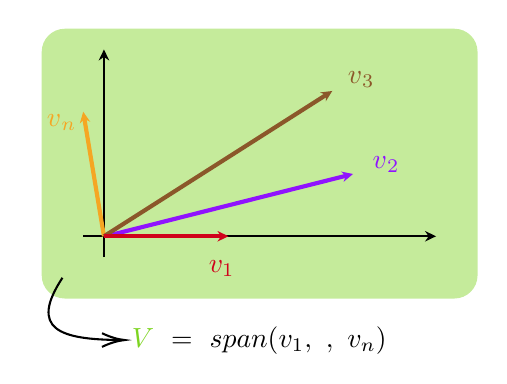
\begin{tikzpicture}[x=0.75pt,y=0.75pt,yscale=-1,xscale=1]
        %uncomment if require: \path (0,300); %set diagram left start at 0, and has height of 300
        %Rounded Rect [id:dp8820310554370777] 
        \draw  [draw opacity=0][fill={rgb, 255:red, 126; green, 211; blue, 33 }  ,fill opacity=0.45 ] (230,31.18) .. controls (230,25.01) and (235.01,20) .. (241.18,20) -- (428.82,20) .. controls (434.99,20) and (440,25.01) .. (440,31.18) -- (440,138.82) .. controls (440,144.99) and (434.99,150) .. (428.82,150) -- (241.18,150) .. controls (235.01,150) and (230,144.99) .. (230,138.82) -- cycle ;
        %Straight Lines [id:da8724031977000506] 
        \draw [color={rgb, 255:red, 144; green, 19; blue, 254 }  ,draw opacity=1 ]  [line width=1.5] (261.02,119.94) -- (377.09,90.73) ;
        \draw [shift={(380,90)}, rotate = 165.88] [fill={rgb, 255:red, 144; green, 19; blue, 254 }  ,fill opacity=1 ][line width=0.08]  [draw opacity=0] (5.36,-2.57) -- (0,0) -- (5.36,2.57) -- (3.56,0) -- cycle    ;
        %Curve Lines [id:da8162772786950714] 
        \draw    (240,140) .. controls (223.75,164.81) and (238.47,169.79) .. (268.16,169.99) ;
        \draw [shift={(270,170)}, rotate = 180.04]  [color={rgb, 255:red, 0; green, 0; blue, 0 }  ][line width=0.75]    (10.93,-3.29) .. controls (6.95,-1.4) and (3.31,-0.3) .. (0,0) .. controls (3.31,0.3) and (6.95,1.4) .. (10.93,3.29)   ;
        %Straight Lines [id:da8087387944084966] 
        \draw [color={rgb, 255:red, 0; green, 0; blue, 0 }  ,draw opacity=1 ]   (250,120) -- (417,120) ;
        \draw [shift={(420,120)}, rotate = 180] [fill={rgb, 255:red, 0; green, 0; blue, 0 }  ,fill opacity=1 ][line width=0.08]  [draw opacity=0] (5.36,-2.57) -- (0,0) -- (5.36,2.57) -- (3.56,0) -- cycle    ;
        %Straight Lines [id:da15624628815900554] 
        \draw [color={rgb, 255:red, 0; green, 0; blue, 0 }  ,draw opacity=1 ]   (260,130) -- (260,33) ;
        \draw [shift={(260,30)}, rotate = 90] [fill={rgb, 255:red, 0; green, 0; blue, 0 }  ,fill opacity=1 ][line width=0.08]  [draw opacity=0] (5.36,-2.57) -- (0,0) -- (5.36,2.57) -- (3.56,0) -- cycle    ;
        %Straight Lines [id:da5317230549382236] 
        \draw [color={rgb, 255:red, 245; green, 166; blue, 35 }  ,draw opacity=1 ] [line width=1.5]  (260,120) -- (250.49,62.96) ;
        \draw [shift={(250,60)}, rotate = 80.54] [fill={rgb, 255:red, 245; green, 166; blue, 35 }  ,fill opacity=1 ][line width=0.08]  [draw opacity=0] (5.36,-2.57) -- (0,0) -- (5.36,2.57) -- (3.56,0) -- cycle    ;
        %Straight Lines [id:da9232604401778618] 
        \draw [color={rgb, 255:red, 139; green, 87; blue, 42 }  ,draw opacity=1 ] [line width=1.5]  (260,120) -- (367.47,51.61) ;
        \draw [shift={(370,50)}, rotate = 147.53] [fill={rgb, 255:red, 139; green, 87; blue, 42 }  ,fill opacity=1 ][line width=0.08]  [draw opacity=0] (5.36,-2.57) -- (0,0) -- (5.36,2.57) -- (3.56,0) -- cycle    ;
        %Straight Lines [id:da30775464381371354] 
        \draw [color={rgb, 255:red, 208; green, 2; blue, 27 }  ,draw opacity=1 ]  [line width=1.5] (260,120) -- (317,120) ;
        \draw [shift={(320,120)}, rotate = 180] [fill={rgb, 255:red, 208; green, 2; blue, 27 }  ,fill opacity=1 ][line width=0.08]  [draw opacity=0] (5.36,-2.57) -- (0,0) -- (5.36,2.57) -- (3.56,0) -- cycle    ;
        % Text Node
        \draw (309,130) node [anchor=north west][inner sep=0.75pt]  [color={rgb, 255:red, 208; green, 2; blue, 27 }  ,opacity=1 ] [align=left] {$\displaystyle v_{1}$};
        % Text Node
        \draw (388,80) node [anchor=north west][inner sep=0.75pt]  [color={rgb, 255:red, 208; green, 2; blue, 27 }  ,opacity=1 ] [align=left] {$\displaystyle \textcolor[rgb]{0.56,0.07,1}{v}\textcolor[rgb]{0.56,0.07,1}{_{2}}$};
        % Text Node
        \draw (376,39) node [anchor=north west][inner sep=0.75pt]  [color={rgb, 255:red, 208; green, 2; blue, 27 }  ,opacity=1 ] [align=left] {$\displaystyle \textcolor[rgb]{0.55,0.34,0.16}{v}\textcolor[rgb]{0.55,0.34,0.16}{_{3}}$};
        % Text Node
        \draw (231,60) node [anchor=north west][inner sep=0.75pt]  [color={rgb, 255:red, 245; green, 166; blue, 35 }  ,opacity=1 ] [align=left] {$\displaystyle \textcolor[rgb]{0.96,0.65,0.14}{v}\textcolor[rgb]{0.96,0.65,0.14}{_{n}}$};
        % Text Node
        \draw (272,162) node [anchor=north west][inner sep=0.75pt]   [align=left] {$\displaystyle \textcolor[rgb]{0.49,0.83,0.13}{V} \ =\ span( v_{1} ,\ \dotsc ,\ v_{n})$};
    \end{tikzpicture}
\end{figure*}

Wenn alle Vektoren \( v_1, \dots, v_n \) eines Erzeugendensystems linear unabhängig sind, dann bilden sie eine Basis. Die Vektoren heissen dann Basisvektoren. 

\vspace{1\baselineskip}

In 2-D wird oft die Standardbasis verwendet. Diese besteht aus den Vektoren 

\begin{equation*}
    \vec{e}_x = \begin{pmatrix} 1 \\ 0 \end{pmatrix} \text{und} \ \vec{e}_y = \begin{pmatrix} 0 \\ 1 \end{pmatrix}. 
\end{equation*}

Jeder 2-D Vektor kann eindeutig als Linearkombination dieser beiden Basisvektoren dargestellt werden. Wir können jedoch auch zwei andere, linear unabhängige, Vektoren als Basisvektoren verwenden. Seien beispielsweise

\begin{equation*}
    \vec{e}_\eta = \begin{pmatrix} 2 \\ 1 \end{pmatrix} \text{und} \ \vec{e}_\zeta = \begin{pmatrix} 1 \\ 2 \end{pmatrix},
\end{equation*}

auch hier können wir jeden 2-D Vektor eindeutig als Linearkombination dieser beiden Vektoren darstellen. Beide Basen beschreiben hier also denselben Vektorraum. Wir sehen, dass die Anzahl von Basisvektoren erhalten bleibt. Die Anzahl an Basisvektoren nennt man Dimension. In unserem Fall mit \( V = \text{span}(\vec{e}_x, \vec{e}_y) = \text{span}(\vec{e}_\eta, \vec{e}_\zeta) \) hat der Vektorraum \( V \) die Dimension 2. Es ist also möglich mehrere Basen für einen endlichdimensionalen Vektorraum zu finden.

\begin{figure*}[!ht]
    \centering
    \tikzset{every picture/.style={line width=0.75pt}} %set default line width to 0.75pt  
    \tikzsetnextfilename{basis_visualisierung}       
    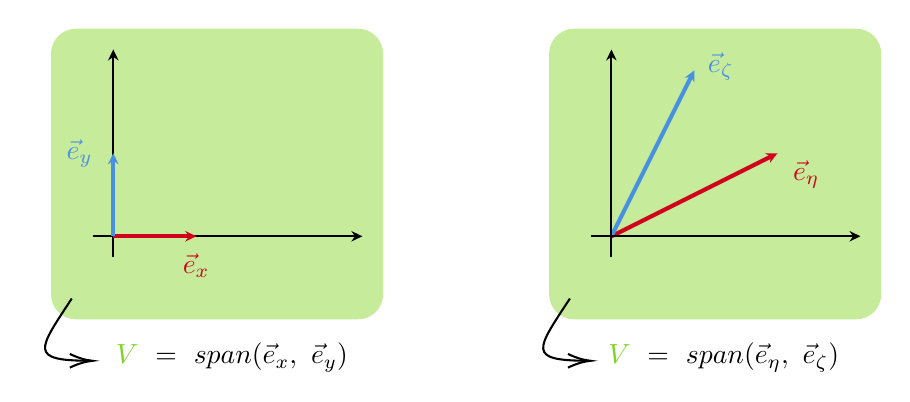
\begin{tikzpicture}[x=0.75pt,y=0.75pt,yscale=-1,xscale=1]
        %uncomment if require: \path (0,340); %set diagram left start at 0, and has height of 340
        %Rounded Rect [id:dp6480805861276174] 
        \draw  [draw opacity=0][fill={rgb, 255:red, 126; green, 211; blue, 33 }  ,fill opacity=0.45 ] (120,32.04) .. controls (120,25.39) and (125.39,20) .. (132.04,20) -- (267.96,20) .. controls (274.61,20) and (280,25.39) .. (280,32.04) -- (280,147.96) .. controls (280,154.61) and (274.61,160) .. (267.96,160) -- (132.04,160) .. controls (125.39,160) and (120,154.61) .. (120,147.96) -- cycle ;
        %Curve Lines [id:da15502106878479371] 
        \draw    (130,150) .. controls (113.75,174.81) and (109.26,179.79) .. (138.19,179.99) ;
        \draw [shift={(140,180)}, rotate = 180.04] [color={rgb, 255:red, 0; green, 0; blue, 0 }  ][line width=0.75]    (10.93,-3.29) .. controls (6.95,-1.4) and (3.31,-0.3) .. (0,0) .. controls (3.31,0.3) and (6.95,1.4) .. (10.93,3.29)   ;
        %Rounded Rect [id:dp7441036731006546] 
        \draw  [draw opacity=0][fill={rgb, 255:red, 126; green, 211; blue, 33 }  ,fill opacity=0.45 ] (360,32.04) .. controls (360,25.39) and (365.39,20) .. (372.04,20) -- (507.96,20) .. controls (514.61,20) and (520,25.39) .. (520,32.04) -- (520,147.96) .. controls (520,154.61) and (514.61,160) .. (507.96,160) -- (372.04,160) .. controls (365.39,160) and (360,154.61) .. (360,147.96) -- cycle ;
        %Straight Lines [id:da8576844833248906] 
        \draw [color={rgb, 255:red, 208; green, 2; blue, 27 }  ,draw opacity=1 ] [line width=1.5]  (390,120) -- (467.32,81.34) ;
        \draw [shift={(470,80)}, rotate = 153.43] [fill={rgb, 255:red, 208; green, 2; blue, 27 }  ,fill opacity=1 ][line width=0.08]  [draw opacity=0] (5.36,-2.57) -- (0,0) -- (5.36,2.57) -- (3.56,0) -- cycle    ;
        %Curve Lines [id:da7023978633292325] 
        \draw    (370,150) .. controls (353.75,174.81) and (349.26,179.79) .. (378.19,179.99) ;
        \draw [shift={(380,180)}, rotate = 180.04] [color={rgb, 255:red, 0; green, 0; blue, 0 }  ][line width=0.75]    (10.93,-3.29) .. controls (6.95,-1.4) and (3.31,-0.3) .. (0,0) .. controls (3.31,0.3) and (6.95,1.4) .. (10.93,3.29)   ;
        %Straight Lines [id:da0540334433374271] 
        \draw [color={rgb, 255:red, 74; green, 144; blue, 226 }  ,draw opacity=1 ] [line width=1.5]  (390,120) -- (428.66,42.68) ;
        \draw [shift={(430,40)}, rotate = 116.57] [fill={rgb, 255:red, 74; green, 144; blue, 226 }  ,fill opacity=1 ][line width=0.08]  [draw opacity=0] (5.36,-2.57) -- (0,0) -- (5.36,2.57) -- (3.56,0) -- cycle    ;
        %Straight Lines [id:da4883835747236054] 
        \draw [color={rgb, 255:red, 0; green, 0; blue, 0 }  ,draw opacity=1 ]   (150,130) -- (150,33) ;
        \draw [shift={(150,30)}, rotate = 90] [fill={rgb, 255:red, 0; green, 0; blue, 0 }  ,fill opacity=1 ][line width=0.08]  [draw opacity=0] (5.36,-2.57) -- (0,0) -- (5.36,2.57) -- (3.56,0) -- cycle    ;
        %Straight Lines [id:da7588620560716264] 
        \draw [color={rgb, 255:red, 0; green, 0; blue, 0 }  ,draw opacity=1 ] (140,120) -- (267,120) ;
        \draw [shift={(270,120)}, rotate = 180] [fill={rgb, 255:red, 0; green, 0; blue, 0 }  ,fill opacity=1 ][line width=0.08]  [draw opacity=0] (5.36,-2.57) -- (0,0) -- (5.36,2.57) -- (3.56,0) -- cycle    ;
        %Straight Lines [id:da0855031246741359] 
        \draw [color={rgb, 255:red, 208; green, 2; blue, 27 }  ,draw opacity=1 ] [line width=1.5]  (150,120) -- (187,120) ;
        \draw [shift={(190,120)}, rotate = 180] [fill={rgb, 255:red, 208; green, 2; blue, 27 }  ,fill opacity=1 ][line width=0.08]  [draw opacity=0] (5.36,-2.57) -- (0,0) -- (5.36,2.57) -- (3.56,0) -- cycle    ;
        %Straight Lines [id:da7935972124804265] 
        \draw [color={rgb, 255:red, 74; green, 144; blue, 226 }  ,draw opacity=1 ] [line width=1.5]  (150,120) -- (150,83) ;
        \draw [shift={(150,80)}, rotate = 90] [fill={rgb, 255:red, 74; green, 144; blue, 226 }  ,fill opacity=1 ][line width=0.08]  [draw opacity=0] (5.36,-2.57) -- (0,0) -- (5.36,2.57) -- (3.56,0) -- cycle    ;
        %Straight Lines [id:da8114402925072283] 
        \draw [color={rgb, 255:red, 0; green, 0; blue, 0 }  ,draw opacity=1 ]   (390,130) -- (390,33) ;
        \draw [shift={(390,30)}, rotate = 90] [fill={rgb, 255:red, 0; green, 0; blue, 0 }  ,fill opacity=1 ][line width=0.08]  [draw opacity=0] (5.36,-2.57) -- (0,0) -- (5.36,2.57) -- (3.56,0) -- cycle    ;
        %Straight Lines [id:da36950183760463695] 
        \draw [color={rgb, 255:red, 0; green, 0; blue, 0 }  ,draw opacity=1 ]   (380,120) -- (507,120) ;
        \draw [shift={(510,120)}, rotate = 180] [fill={rgb, 255:red, 0; green, 0; blue, 0 }  ,fill opacity=1 ][line width=0.08]  [draw opacity=0] (5.36,-2.57) -- (0,0) -- (5.36,2.57) -- (3.56,0) -- cycle    ;
        % Text Node
        \draw (126,72) node [anchor=north west][inner sep=0.75pt]  [color={rgb, 255:red, 74; green, 144; blue, 226 }  ,opacity=1 ] [align=left] {$\displaystyle \textcolor[rgb]{0.29,0.56,0.89}{\vec{e}}\textcolor[rgb]{0.29,0.56,0.89}{_{y}}$};
        % Text Node
        \draw (149.88,170) node [anchor=north west][inner sep=0.75pt]   [align=left] {$\displaystyle \textcolor[rgb]{0.49,0.83,0.13}{V} \ =\ span(\vec{e}_{x} ,\ \vec{e}_{y})$};
        % Text Node
        \draw (182,127) node [anchor=north west][inner sep=0.75pt]  [color={rgb, 255:red, 245; green, 166; blue, 35 }  ,opacity=1 ] [align=left] {$\displaystyle \textcolor[rgb]{0.82,0.01,0.11}{\vec{e}}\textcolor[rgb]{0.82,0.01,0.11}{_{x}}$};
        % Text Node
        \draw (435,30) node [anchor=north west][inner sep=0.75pt]  [color={rgb, 255:red, 74; green, 144; blue, 226 }  ,opacity=1 ] [align=left] {$\displaystyle \textcolor[rgb]{0.29,0.56,0.89}{\vec{e}}\textcolor[rgb]{0.29,0.56,0.89}{_{\zeta }}$};
        % Text Node
        \draw (387,170) node [anchor=north west][inner sep=0.75pt]   [align=left] {$\displaystyle \textcolor[rgb]{0.49,0.83,0.13}{V} \ =\ span(\vec{e}_{\eta } ,\ \vec{e}_{\zeta })$};
        % Text Node
        \draw (476,82) node [anchor=north west][inner sep=0.75pt]  [color={rgb, 255:red, 245; green, 166; blue, 35 }  ,opacity=1 ] [align=left] {$\displaystyle \textcolor[rgb]{0.82,0.01,0.11}{\vec{e}}\textcolor[rgb]{0.82,0.01,0.11}{_{\eta }}$};
    \end{tikzpicture}
\end{figure*}

Versuchen wir nun einen spezifischen Vektor in der Standardbasis \( \vec{e}_x, \vec{e}_y \) und der Basis \( \vec{e}_\eta, \vec{e}_\zeta \) auszudrücken. Betrachten wir hierfür zunächst den Vektor 

\begin{equation*}
    \begin{pmatrix} 3 \\ 3 \end{pmatrix} = \sum_{i=1}^{n} x_i v_i. 
\end{equation*}


\vspace{1\baselineskip}

In der Standardbasis suchen wir also \( x_1, x_2 \) sodass

\begin{equation*}
    \begin{pmatrix} 3 \\ 3 \end{pmatrix} = x_1 \begin{pmatrix} 1 \\ 0 \end{pmatrix} + x_2 \begin{pmatrix} 0 \\ 1 \end{pmatrix}.
\end{equation*}

Wir erkennen sofort, dass \( x_1 = x_2 = 3 \) sein muss. Somit ist der Koordinatenvektor bezüglich der Standardbasis \( \vec{e}_x, \vec{e}_y \): 

\begin{equation*}
    \begin{pmatrix} 3 \\ 3 \end{pmatrix}_{x,y}. 
\end{equation*}

In der Basis \( \vec{e}_\eta, \vec{e}_\zeta \) suchen wir nun \( x_1, x_2 \) sodass

\begin{equation*}
    \begin{pmatrix} 3 \\ 3 \end{pmatrix} = x_1 \begin{pmatrix} 2 \\ 1 \end{pmatrix} + x_2 \begin{pmatrix} 1 \\ 2 \end{pmatrix}.
\end{equation*}

Hier erkennen wir sofort, dass \( x_1 = x_2 = 1 \) sein muss. Somit ist der Koordinatenvektor bezüglich der Basis \( \vec{e}_\eta, \vec{e}_\zeta \):

\begin{equation*}
    \begin{pmatrix} 1 \\ 1 \end{pmatrix}_{\eta, \zeta}.
\end{equation*}

Der Koordinatenvektor hängt also immer von der gewählten Basis ab!

\newpage
\section{Lineare Abbildungen}  

\begin{tcolorbox}[colback=gray!30, colframe=gray!80, title=Lineare Abbildung]
Seien \( V, W \) reelle Vektorräume. Dann heisst

\begin{equation*}
    \mathcal{F}: V \rightarrow W, \quad x \mapsto \mathcal{F}(x)
\end{equation*}

\vspace{0.5\baselineskip}

lineare Abbildung, falls \( \forall x, y \in V, \ \forall \alpha \in \mathbb{R} \) gilt:

\begin{equation*}
    \begin{aligned}
        i. \quad \mathcal{F}(x + y) &= \mathcal{F}(x) + \mathcal{F}(y) \\
        ii. \quad \mathcal{F}(\alpha x) &= \alpha \mathcal{F}(x).
    \end{aligned}
\end{equation*}
\end{tcolorbox}

\vspace{0.5\baselineskip}

Wenn wir nun prüfen wollen, ob eine Abbildung linear ist, dann müssen wir prüfen ob i.\ und ii.\ erfüllt sind. Als Beispiel betrachten wir die Abbildung

\begin{equation*}
    \mathcal{F}: \mathbb{R} \rightarrow \mathbb{R}, \quad x \mapsto 3x. 
\end{equation*}

\vspace{0.5\baselineskip}

Wir prüfen nun i.\ und ii.\ für diese Abbildung:

\begin{equation*}
    \begin{aligned}
        i. \quad \mathcal{F}(x + y) &= 3(x + y) = 3x + 3y = \mathcal{F}(x) + \mathcal{F}(y) \\
        ii. \quad \mathcal{F}(\alpha x) &= 3(\alpha x) = \alpha \cdot 3x = \alpha \cdot \mathcal{F}(x).
    \end{aligned}
\end{equation*}

\vspace{0.5\baselineskip}

In diesem Fall ist die Abbildung \( \mathcal{F} \) linear. 

\vspace{1\baselineskip}

Aus den Bedingungen i.\ und ii.\ foglen bestimmte Eigenschaften die jede lineare Abbildung besitzt. So wird z.B. der Nullvektor immer auf den Nullvektor abgebildet. Wenn ausserdem \( V, W \) endlichdimensionale Vektorräume sind, z.B. \( V = \mathbb{R}^n, W = \mathbb{R}^m \), dann kann jede lineare Abbildung \( \mathcal{F}: V \rightarrow W \)  durch eine Matrix \( A \in \mathbb{R}^{m \times n} \) dargestellt werden. Allgemein kann man eine lineare Abbildung in der Form

\begin{equation*}
    \mathcal{F}: \mathbb{R}^n \rightarrow \mathbb{R}^m, \quad x \mapsto Ax
\end{equation*}

\vspace{0.5\baselineskip}

schreiben, wobei \( A \in \mathbb{R}^{m \times n} \) die Abbildungsmatrix von \( \mathcal{F} \) ist. Als Beispiel betrachten wir die Abbildung \( \mathcal{F} \) gegeben durch

\begin{equation*}
    \mathcal{F}: \mathbb{R}^2 \rightarrow \mathbb{R}^3, \quad \begin{pmatrix} x \\ y \end{pmatrix} \mapsto \begin{pmatrix} x + y \\ x - 2y \\ 3x \end{pmatrix}.
\end{equation*}

\vspace{0.5\baselineskip}

Wir können die Abbildung in die Form \( x \mapsto Ax \) bringen, indem wir die Abbildungsmatrix \( A \) bestimmen. In diesem Fall ist

\begin{equation*}
    \begin{pmatrix} x \\ y \end{pmatrix} \mapsto \begin{pmatrix} x + y \\ x - 2y \\ 3x \end{pmatrix} = \underbrace{\begin{pmatrix} 1 & 1 \\ 1 & -2 \\ 3 & 0 \end{pmatrix}}_{:=A} \begin{pmatrix} x \\ y \end{pmatrix}.
\end{equation*}